\documentclass[11pt]{article}


\usepackage{tristan-quick-note}


\def\CourseName{Cryptography}
\def\CourseNumber{388}
\def\Assignment{Midterm}
\def\AssignmentNumber{1}
\def\DueDate{October 1st, 2018}
\def\CenterHeader{}
\def\Name{Tristan Wylde-LaRue}
\def\RightHeader{An Introduction to Quantum Computing}

\usetikzlibrary{arrows, shapes.gates.logic.US, calc}
\usepackage{braket}

\begin{document}

% \textbf{Some background:} Quantum Mechanics came into prevalence in the early 1900s. 




\begin{center}
\textbf{\Large Classical Computing and Classical Information} \\
\end{center}
\bigskip

\textbf{The Bit} \\
The fundamental unit of information is the bit. The term bit was introduced by Claude Shannon in 1948. It was a contraction of ``binary information digit''. A bit is the smallest nontrivial unit of information.

A bit $b$ has two possible states. Generally, this is represented as
\[
    b \in \{0, 1\} \simeq \{\text{True},\ \text{False}\} \simeq \Z/2\Z
\]
Sometimes thinking of a bit as true/false is helpful.

Importantly, we can have a list of several bits. A string $s$ (of length $n$) is an ordered tuple of $n$-bits. This is expressed as a cartesian product
\[
    s \in \{0, 1\}^n \simeq (\Z/2\Z)^n
\]

\pagebreak

\textbf{Logic Gates and Bit Operations} \\
We can perform operations on bits. We will express these as logic gates. If you've done propositional logic in a philosphy or math class, this is the same system just with different notation.

We start with the unary gates. These take one bit as input and return one bit. Here is a $\texttt{NOT}$ gate:
\begin{center}
    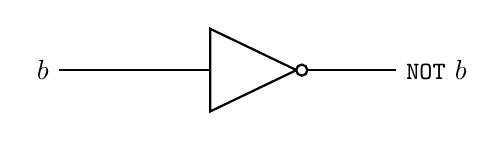
\begin{tikzpicture}[thick]
        \node (b) at (0, 0) {$b$};
        \node (bout) at (5,0) {\texttt{\small NOT} $b$};
        \node[not gate US, draw, minimum size=0.9cm] at ($(b) + (2.5, 0)$) (notb) {};
        \draw (b) -- (notb.input);
        \draw (notb.output) -- (bout);
    \end{tikzpicture}
    \hphantom{XXXX}
\end{center}

It takes 0 to 1 and 1 to 0. It can be defined by the truth table:
\begin{tabular}{l|l}
0 & 1 \\
1 & 0
\end{tabular}

There are in fact 4 unary gates, one for each of the 4 truth tables. Writing them out is a good exercise. Importantly More generally, the logic of any circuit is nothing more or less than a truth table. Here is an arbitary circuit:
\begin{center}
    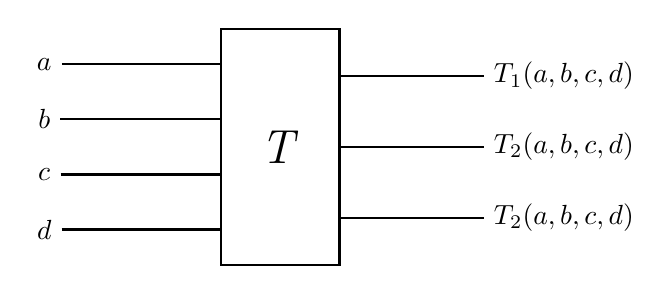
\begin{tikzpicture}[thick]
        \node (a) at (1, 3.05) {$a$};
        \node (b) at (1, 2.35) {$b$};
        \node (c) at (1, 1.65) {$c$};
        \node (d) at (1, 0.95) {$d$};

        \node (x) at (7.6, 2.9) {$T_1(a, b, c, d)$};
        \node (y) at (7.6, 2) {$T_2(a, b, c, d)$};
        \node (z) at (7.6, 1.1) {$T_2(a, b, c, d)$};

        \node (rect) at (4,2) [draw,thick,minimum width=1.5cm,minimum height=3cm] {\textit{\LARGE T}};

        \draw (a) -- (3.24, 3.05);
        \draw (b) -- (3.24, 2.35);
        \draw (c) -- (3.24, 1.65);
        \draw (d) -- (3.24, 0.95);
        \draw (4.76, 2.9) -- (x);
        \draw (4.76, 2) -- (y);
        \draw (4.76, 1.1) -- (z);
    \end{tikzpicture}
\end{center}
In this case $T : \{0,1\}^4 \rightarrow \{0,1\}^3$ takes as input 4 bits and returns 3 bits. I use the variable $T$ to emphasize that could be thought of as a truth table.



There are two-bit gates $\texttt{AND}$ and $\texttt{XOR}$. The fancy symbol here $\oplus$ means $\texttt{XOR}$. It gets a special symbol because it has the special property of being linear. \\

\begin{halfpage}
    \centering
    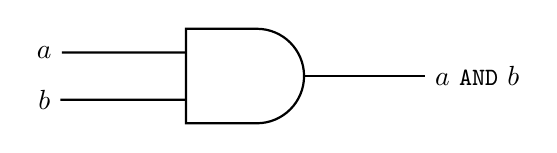
\begin{tikzpicture}[thick]
        \node (x) at (0, 0.8) {$a$};
        \node (y) at (0, 0.2) {$b$};
        \node (output) at (5.5,0.5) {$a$ \texttt{\small AND} $b$};

        \node[and gate US, draw, rotate=0, logic gate inputs=222, minimum size=1.2cm] at ($(2.5, 0.5)$) (xory) {};
        \draw (x) -- (xory.input 1);
        \draw (y) -- (xory.input 3);

        \draw (xory.output) -- (output);
    \end{tikzpicture}
\end{halfpage}
\begin{halfpage}
    \centering
    \begin{tikzpicture}[thick]
        \node (x) at (0, 0.8) {$a$};
        \node (y) at (0, 0.2) {$b$};
        \node (output) at (5.5,0.5) {$a$ \oplus \  $b$};


        \node[xor gate US, draw, rotate=0, logic gate inputs=22, minimum size=1.2cm] at ($(2.5, 0.5)$) (xory) {};
        \draw (x) -- (1.74, 0.8);
        \draw (y) -- (1.74, 0.2);

        \draw (xory.output) -- (output);
    \end{tikzpicture}
\end{halfpage}

I should mention that you can build any arbitrary circuit using \texttt{AND} and \texttt{NOT}.\,  Here are two examples, \texttt{Controlled AND} and \texttt{Controlled XOR} \\


    \begin{halfpage}
    

    \begin{center}
      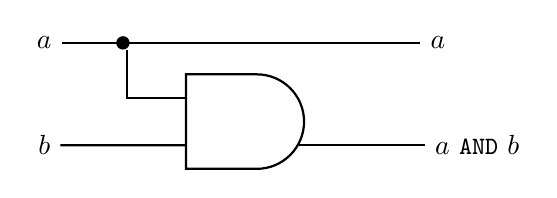
\begin{tikzpicture}[thick]
        \node (x) at (0, 1.5) {$a$};
        \node (y) at (0, 0.2) {$b$};
        \node[circle, fill=black, inner sep=0pt, minimum size=1.7mm] (c) at (1, 1.5) {};
        \node (output) at (5.5,0.2) {$a$ \texttt{\small AND} $b$};
        \node (aout) at (5,1.5){$a$};
 
        \node[and gate US, draw, rotate=0, logic gate inputs=222, minimum size=1.2cm] at ($(2.5, 0.5)$) (xory) {};
        \draw (x) -- (c);
        \draw (c) -- ([xshift=0.4cm]c) |- (xory.input 1);
        \draw (y) -- (xory.input 3);
        \draw (x) -- (aout);
        \draw (3.23,0.2) -- (output);
    \end{tikzpicture}
    \end{center}
    \end{halfpage}
    \begin{halfpage}
    \begin{center}
            \begin{tikzpicture}[thick]
        \node (x) at (0, 1.5) {$a$};
        \node (y) at (0, 0.2) {$b$};
        \node (aout) at (5,1.5){$a$};
        \node (output) at (5.5,0.5) {$a$ \oplus \  $b$};
        \node[circle, fill=black, inner sep=0pt, minimum size=1.7mm] (c) at (1, 1.5) {};

        \node[xor gate US, draw, rotate=0, logic gate inputs=22, minimum size=1.2cm] at ($(2.5, 0.5)$) (xory) {};
        \draw (x) -- (c);
        \draw (c) -- (aout);
        \draw (y) -- (1.74, 0.2);
        \draw (c) -- ([xshift=0.4cm]c) |- (1.74, 0.8);
        \draw (xory.output) -- (output);
    \end{tikzpicture}
    \end{center}
     \end{halfpage}

    The second one, \texttt{Controlled XOR} is $\textit{reversible}$. If we apply it twice, we get the identity. Such gates are classically important because they don't add entropy and thus generate less heat.

    \pagebreak

    \begin{center}
        \textbf{\Large Quantum Computing and Quantum Information} \\
    \end{center}
        \bigskip 

    \textbf{The Qubit} \\
    \textit{Background: Just as the bit is the fundamental unit of information, the qubit is the fundamental unit of quantum information. It represents the state of a 2 state quantum mechanical system (the simplest nontrivial quantum system)}

    A classical bit is either 0 or 1. A qubit is a pair of complex numbers 
    \[
        (\alpha, \beta) \in \C^2 
    \]
    satisfying the condition
    \[
        |\alpha|^2 + |\beta|^2 = 1
    \]
    Importantly, $\C^2$ is a 2-dimensional vector space and so it has a basis. There is o    \[
        \left\{\cvec{0}{1}, \cvec{1}{0}\right\}
    \]
    which we will call $\ket{0}$ and $\ket{1}$, using the physics notation.\\ 

    Why does it live in $\C^2$? That's what the physicists tell me. \\ 
    This does raise an issue though. $\C^2$ is a continuous vector space. This means that we couldn't even write down the state of a qubit in a finite number of classical bits.


\end{document}